\section{Protocolo para control de cartel luminoso}\label{sec:protocolo}

\subsection{Codificación}
Cada mensaje del protocolo es un paquete de tamaño variable, con un límite máximo de 256 octetos. (Incluyendo todos los headers)

Todos los valores numéricos se transmiten con orden de bytes Big-Endian.

Cada mensaje respeta un formato base común. Se puede ver este formato en la figura \ref{fig:paquete-base}.

\begin{figure}[h]
	\centering
	\label{fig:paquete-base}
	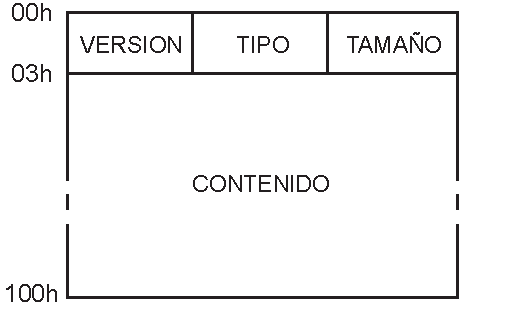
\includegraphics[scale=0.8]{imagenes/paquete-base.pdf}
		\caption{Formato del paquete base.}
\end{figure}

VERSION es un número que identifica la versión del protocolo, por si se hicieran cambios y se quiera mantener retrocompatibilidad.

TIPO es un enumerativo que codifica el tipo de mensaje. TAMAÑO indica el tamaño del mensaje, tiene rango [3, 253].

Un mensaje inválido se descarta y termina la conexión. (bajo TLS, no puede tratarse de corrupción, asi que es un cliente mal implementado o malicioso)

CONTENIDO contiene una estructura que depende de TIPO y se define para cada interacción más adelante.

\subsubsection{Strings}
Los strings tienen un límite de longitud dado por el lugar remanente en el mensaje y están codificados según el estándar ISO/IEC 8859-1:1998. Antes del contenido del string debe haber un byte que indique la longitud del string.

\subsection{Establecimiento de conexión}
El establecimiento de una conexión está conformado por el establecimiento de una conexión TLS al servidor iniciada por el cliente, seguida de la interacción Authenticate. Si la interacción Authenticate fallase, el servidor debe cerrar la conexión inmediatamente.

El acceso al servidor dura lo que dure la conexión; no debe mantenerse estado de autenticación fuera de una conexión.

\subsection{Desconexión}
La desconexión es sólo la de TLS. Una desconexión a nivel TCP sin la interacción de desconexión de TLS se considera un error.

\subsection{Interacciones}
Una interacción es una secuencia de dos mensajes: un mensaje de pedido y un mensaje de respuesta. Cada interacción está formada por un mensaje de pedido seguido por un mensaje de respuesta.
Las interacciones posibles son:

\begin{itemize}
	\item Authenticate
	\item SetText
	\item SetAnimationParameters
	\item SetWifiConfiguration
	\item GetText
	\item GetAnimationParameters
	\item GetWifiConfiguration
\end{itemize}

La respuesta proviniente del servidor tiene el siguiente formato de la figura \ref{fig:paquete-respuesta}.

\begin{figure}[h]
	\centering
	\label{fig:paquete-respuesta}
	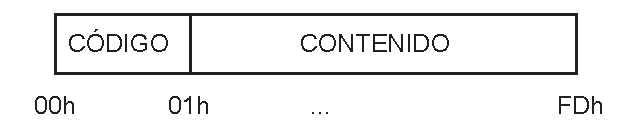
\includegraphics[scale=0.8]{imagenes/paquete-respuesta.pdf}
		\caption{Formato de la respuesta.}
\end{figure}


ResponseCode puede tomar los siguientes valores:
\begin{itemize}
	\item Respuesta genérica indicando éxito: 0
	\item Error genérico: -1
	\item Paquete inválido: -2
	\item Paquete incompatible: -3
	\item Configuración de WiFi inválida: -4
\end{itemize}

El campo CONTENIDO es opcional, puede ser de tamaño nulo y su valor depende de la interacción de la cual es respuesta. Se dice que una interacción tiene una respuesta vacía cuando el campo CONTENIDO está ausente. Toda interacción tiene respuesta vacía salvo que se indique lo contrario.

\subsubsection{Authenticate}
Cuando se inicia la conexión TLS, el cliente manda la contraseña para entrar al sistema. El servidor responde con una respuesta de OK y la conexión permanece establecida hasta que el cliente decida cerrarla. (Cerrar la conexión TLS implica primero señalizar su fin, solo hacer FIN o RST se considera como una intrusión a la conexión y es detectable por ambas partes)

\subsubsection{SetText}
Actualiza el mensaje del cartel con el enviado en el pedido.

El servidor responde con un OK o con un código de error.

Este pedido tiene el formato de la figura \ref{fig:paquete-text}.
\begin{figure}[h]
	\centering
	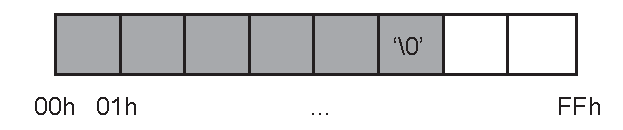
\includegraphics[scale=0.8]{imagenes/paquete-text.pdf}
	\caption{Formato del pedido SetTextRequest.}
	\label{fig:paquete-text}
\end{figure}

En este caso el contenido del mensaje es una string terminada en cero.

\subsubsection{SetAnimationParameters}
Actualiza la configuración de la animación del cartel.

Este pedido tiene el formato de la figura \ref{fig:paquete-animparams}.
\begin{figure}[h]
	\centering
	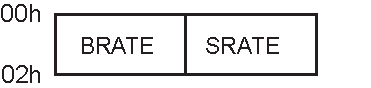
\includegraphics[scale=0.8]{imagenes/paquete-animparams.pdf}
	\caption{Formato del pedido SetAnimationParameters.}
	\label{fig:paquete-animparams}
\end{figure}

BRATE y SRATE son la frequencia de parpadeo en Hz y la velocidad de deslizamiento en píxeles por segundo.

Se asume que si BRATE es cero, no se debe parpadear el contenido. De la misma forma, si SRATE es cero, no se debe deslizar el contenido.

El tipo de dato ufp844 es un número en punto fijo sin signo con 4 bits de parte entera y 4 bits de parte fraccionaria. El tipo de dato sfp844 es lo mismo que ufp844 pero en complemento a dos.

\subsubsection{SetWifiConfiguration}
Actualiza la configuración de WiFi del servidor. En caso de éxito, el servidor debe responder con el código de respuesta de éxito, luego debe cerrar la conexión y por último debe conectarse a la red indicada bajo la IP indicada. Si fallara en hacer eso, vuelve a la configuración anterior.

Este pedido tiene el formato de la figura \ref{fig:paquete-wifi}.
\begin{figure}[h]
	\centering
	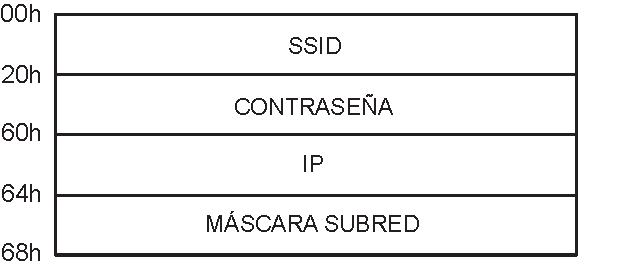
\includegraphics[scale=0.8]{imagenes/paquete-wifi.pdf}
	\caption{Formato del pedido SetWifiConfiguration.}
	\label{fig:paquete-wifi}
\end{figure}

SSID es el nombre de la red, CONTRASEÑA es la contraseña de la red, IP es la IP que va a tomar el cartel y MÁSCARA SUBRED es la máscara de la subred.

\subsubsection{GetText}
Devuelve la estructura correspondiente a SetText con el mensaje actual del cartel.
Siempre retorna código de éxito.

\subsubsection{GetAnimationParameters}
Devuelve la estructura correspondiente a SetAnimationParameters con la configuración de animación actual del cartel.
Siempre retorna código de éxito.

\subsubsection{GetWifiConfiguration}
Devuelve la estructura correspondiente a SetWifiConfiguration con los datos de la red a la que el cartel está conectado y la IP que tiene en ella.
Siempre retorna código de éxito.
